\section{Ingestion-Service}

Wie in \fref{sec:entw-ingestion} beschrieben, wird für ein Event ein Prozess gestartet.
Der Name der Topic des Events zum Starten einer Ingestion ist "`dls\_\_ingestion\_\_run"'.
In \fref{sec:ingestion-run} wird der detailliere Ablauf mit den verschiedenen Wegen für Read- und SaveTypes beschrieben.
Vorher werden die benötigt Grundlagen zur Ausführung erläutert.

\subsection{Berechnen und Speichern der Änderungsdaten}
Um Änderungen in eine Delta Tabelle zu übernehmen, müssen die Änderungsdaten in einem Format sein, dass Aufschluss darüber gibt, welche Daten hinzugefügt, welche geändert und welche gelöscht worden sind.
Das hier verwendete Format muss genau dem gleichen Schema entsprechen, wie die original Daten.
Zusätzlich soll eine Spalte oder ein Feld auf der obersten Eben mit dem Namen "`cd\_deleted"' vorhanden sein.
Es enthält einen Boolean-Wert, der sagt, ob der Eintrag aus den Daten gelöscht wurde oder nicht.
Der Datensatz mit den Änderungsdaten darf außerdem nur geänderte Daten enthalten.
Aus diesem Format können, wie später gezeigt, die drei Operationen abgeleitet werden.

Um nicht auf ein externes Change-Data-Capture-System angewiesen zu sein, gibt es eine interne Lösung, die auf alle (semi-)strukturierten Daten angewendet werden kann.
Der \cref{algo:delta-calc} zeigt, wie aus zwei DataFrames die Änderungsdaten erzeugt werden.
Als Eingabe werden ein linkes DataFrame, mit dem aktuellen internen Stand, eine rechtes DataFrame, mit den neuen Daten und der Name der Id-Spalte benötigt.
Das Ergebnis ist ein DataFrame mit allen aktualisierten Datensätzen.
Es hat das gleiche Schema wie die Ursprungsdaten, aber mit der zusätzlichen Spalte, die Auskunft darüber gibt, ob ein Datensatz gelöscht wurde.

\begin{algorithm}
    \caption{Deltaberechnung}
    \label{algo:delta-calc}
    \KwData{leftDataFrame, rightDataFrame, idColumn}
    \KwResult{changeDataFrame}
    $leftDataFrame \gets$ add column with row hash \;
    $leftDataFrame \gets$ prefix column names with "`left\_"' \;
    $rightDataFrame \gets$ add column with row hash \;
    $rightDataFrame \gets$ prefix columnnames with "`right\_"' \;

    $changeDataFrame \gets$ full join over $idColumn$ of $leftDataFrame$ and $rightDataFrame$ \;

    $changeDataFrame \gets$ remove all rows where $left\_hash$ equals $right\_hash$ \;

    $changeDataFrame \gets$ remove hash columns

    $changeDataFrame \gets$ add row $cd\_deleted$ \;
    \eIf{$right\_idColumn$ is $null$}{$cd\_deleted = true$}{$cd\_deleted = false$}

    $changeDataFrame \gets$ merge left and right $idColumn$ into one $idColumn$
    \eIf{$left\_idColumn$ is not $null$}{$idColumn = left\_idColumn$}{$idColun = right\_idColumn$}

    $changeDataFrame \gets$ merge remaining columns with left and right value by always taking the right and removing prefix

\end{algorithm}

Das Einpflegen der Änderungen wird über die Delta Lake API gelöst.
Dazu werden die Änderungsdaten mit den aktuellen Daten über die Id-Spalte zusammengeführt.
Dabei können verschieden Fälle definiert werden.
Wenn die Ids einer Zeile gleich sind und die Spalte "`cd\_deleted"' $true$ enthält, wird die Zeile aus den Daten gelöscht, ansonsten wird der Datensatz aktualisiert.
Wenn die Ids nicht übereinstimmen und die Spalte "`cd\_deleted'" $false$ ist, dir der Datensatz als neue Zeile eingefügt.

\subsection{Plugins verwalten}
Für jede Ingestion wird auf dem Speichersystem des Mircoservices ein temporärer Ordner angelegt, in den die Plugins und deren Abhängigkeiten installiert werden.
Nach der Installation wird noch eine Datei angelegt, die für alle Pakete die Versionen enthält.
Das dient dazu, bei einer erneuten Ausführung auf dem Service nicht alle Pakete neu installieren zu müssen, sondern nur die mit geänderten Version.
Das beschleunigt die Ausführung der Ingestion.
Zum Schluss wird der Ordner, in den die Pakete installiert wurden an den Python-Pfad mit angehangen.
Damit wird dieser während der Ausführung manipuliert und die Pakete sind verfügbar.
Da jede Ingestion in einem eigenen Prozess beeinflussen die Änderungen an dem Python-Pfad den Ingestion-Service oder andere Prozesse nicht.

Im zweiten Schritt wird jede Python-Datei im Pluginordner als Modul geladen.
Die im Modul verfügbaren Methoden werden dann überprüft, ob sie auf eine Definition der möglichen Plugins passen.
Dazu wird der \fref{algo:check-method} verwendet.
Diesem werden das geladene Modul, ein Name der Methode, ein optionaler Rückgabetyp der Methode und eine Liste von Parameter, bei denen Name und Typ definiert ist.
Zur Überprüfung können alle Methoden in dem Modul auf ihren Namen geprüft werden.
Wenn eine Methode gefunden wurde, wird eine Signatur erzeugt und mit der übergebenen Definition verglichen.
Das Ergebnis sagt dann, ob diese Methode ein Plugin ist oder nicht.

Jedes geladene Modul wird auf Load- oder AfterLoad-Methoden geprüft.
Eine gefundene Load-Methode überschreibt immer die letzte gefunden, da bei einer Ausführung auch das Ergebnis dieser Methoden überschrieben werden würde.
Die AfterLoad-Methoden dagegen werden in einer Liste gespeichert.


\begin{algorithm}
    \caption{Pluginmethode überprüfen}
    \label{algo:check-method}

    \KwData{$plugin$, $name$, $return\_type$, $parameters$}

    \KwResult{$matches$}

    \If{plugin has NOT method with name $name$}{
        \Return{false}
    }

    $signature \gets$ signature of mehtod $name$

    \If{$return\_type$ is given AND $signature$ NOT returns type of $return\_type$}{
        \Return{false}
    }

    \ForAll{$param$ in $parameters$}{
        \If{$signature$ has NOT a parameter named $param.name$}{
            \Return{false}
        }

        \If{$signature$ type of parameter $param.name$ is NOT $parameter.type$}{
            \Return{false}
        }
    }

    \Return{true}

\end{algorithm}

\subsection{Ausführung der Ingestion}
\label{sec:ingestion-run}
Die Ausführung startet mit der Initialisierung, die die für die Ingestion benötigte Daten lädt.
Das ist zum Beispiel die DatasourceDefinition zu der Id aus den Events.
Danach wird entschieden ob eine Ingestion über Spark notwendig ist.
Hier spielt der Lesetyp eine große Rolle.
Eine Ingestion von Datendateien benötigt keine Spark, es werden einfach direkt die Dateien in das entsprechende Zielverzeichnis kopiert.
Für alle anderen Typen wird im nächsten Schritt die Ingestion vorbereitet.
Es werden die Plugins aus dem HDFS geladen und eine SparkSession erstellt.
Das Laden der Daten in ein DataFrame geschieht anschließend entweder über ein Plugin in oder das Standardvorgehen.
Falls auch After-Load-Plugins vorhanden sind werden diese ausgeführt.
Für die geladenen Daten wird dann entschieden, ob es sich um Änderungsdaten handelt oder welche berechnet werden müssen.
Je nach Schreib-Typ werden dann die Daten beziehungsweise Ändeurngsdaten gespeichert.
Für Datenströme wird am Ende noch ein Hintergrund Task gestartet, der auf Kafka Events zum stoppen dieser Ingestion wartet.
Hierfür wird die Topic "`dls\_\_ingestion\_\_stop\_ingestion"' mit der Id als Wert verwendet.
Wenn die Ingestion beendet wurde, wird zum Schluss die SparkSession gestoppt.

\begin{figure}
    \centering
    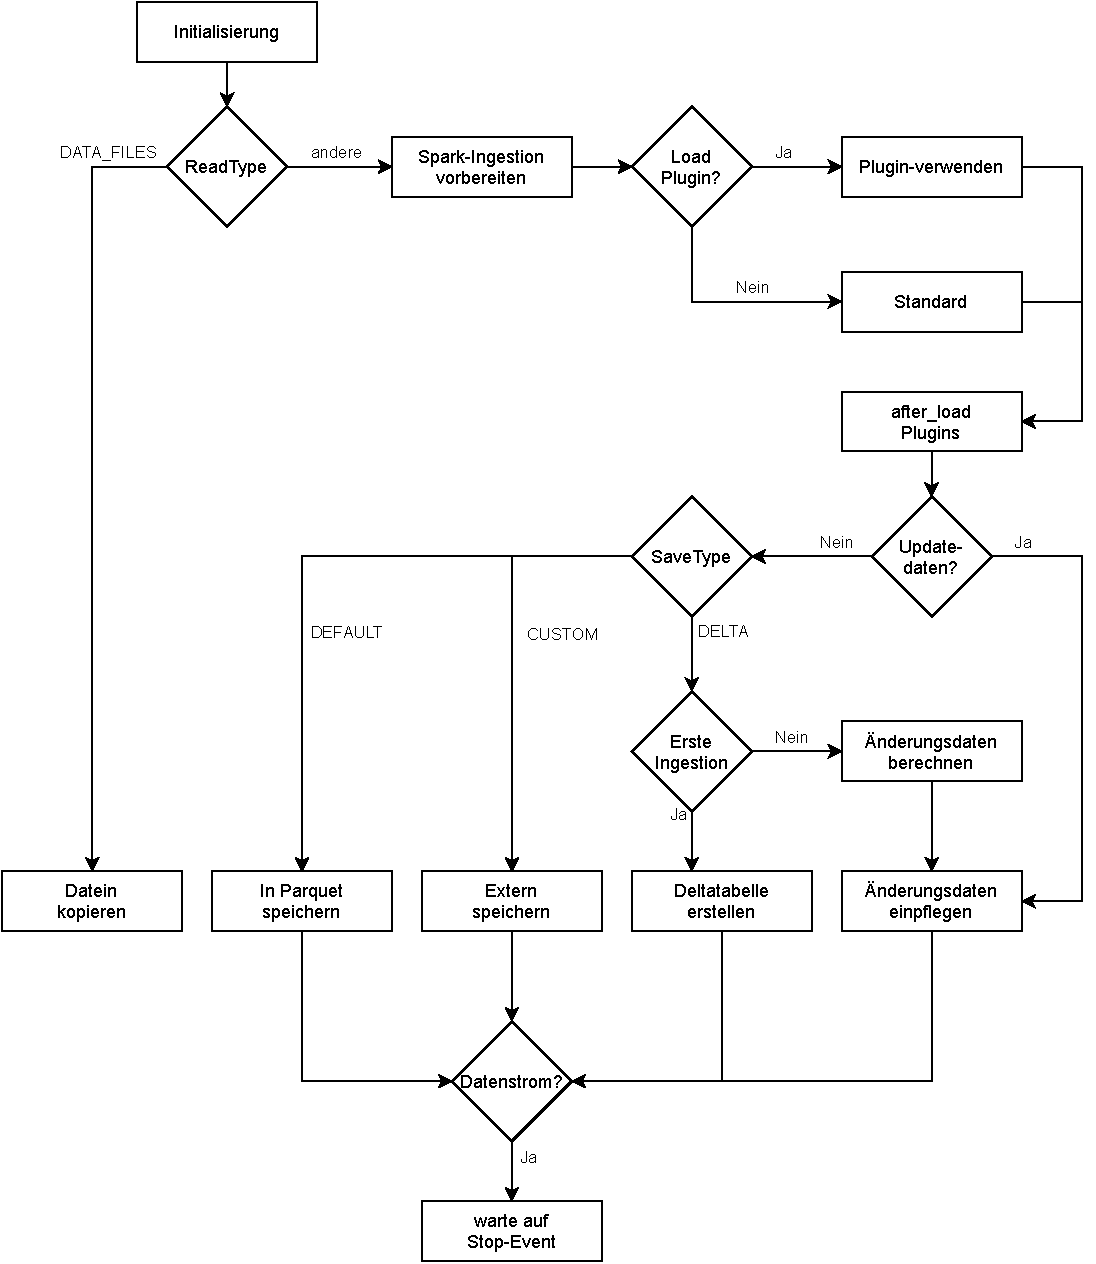
\includegraphics[width=\textwidth]{Grafiken/Umsetzung-Ingestion-Ablauf.pdf}
    \caption{Ablauf einer Ingestion}
    \label{fig:umsetz-ingestion-ablauf}
\end{figure}